\documentclass{article}

\usepackage{graphicx}

\title{MAS AI Assignment 1}
\date{}
\author{Simon Deussen}

\begin{document}
  \pagenumbering{gobble}
  \maketitle
  \pagenumbering{arabic}

\section*{Task 1}
\begin{figure}[h!]
    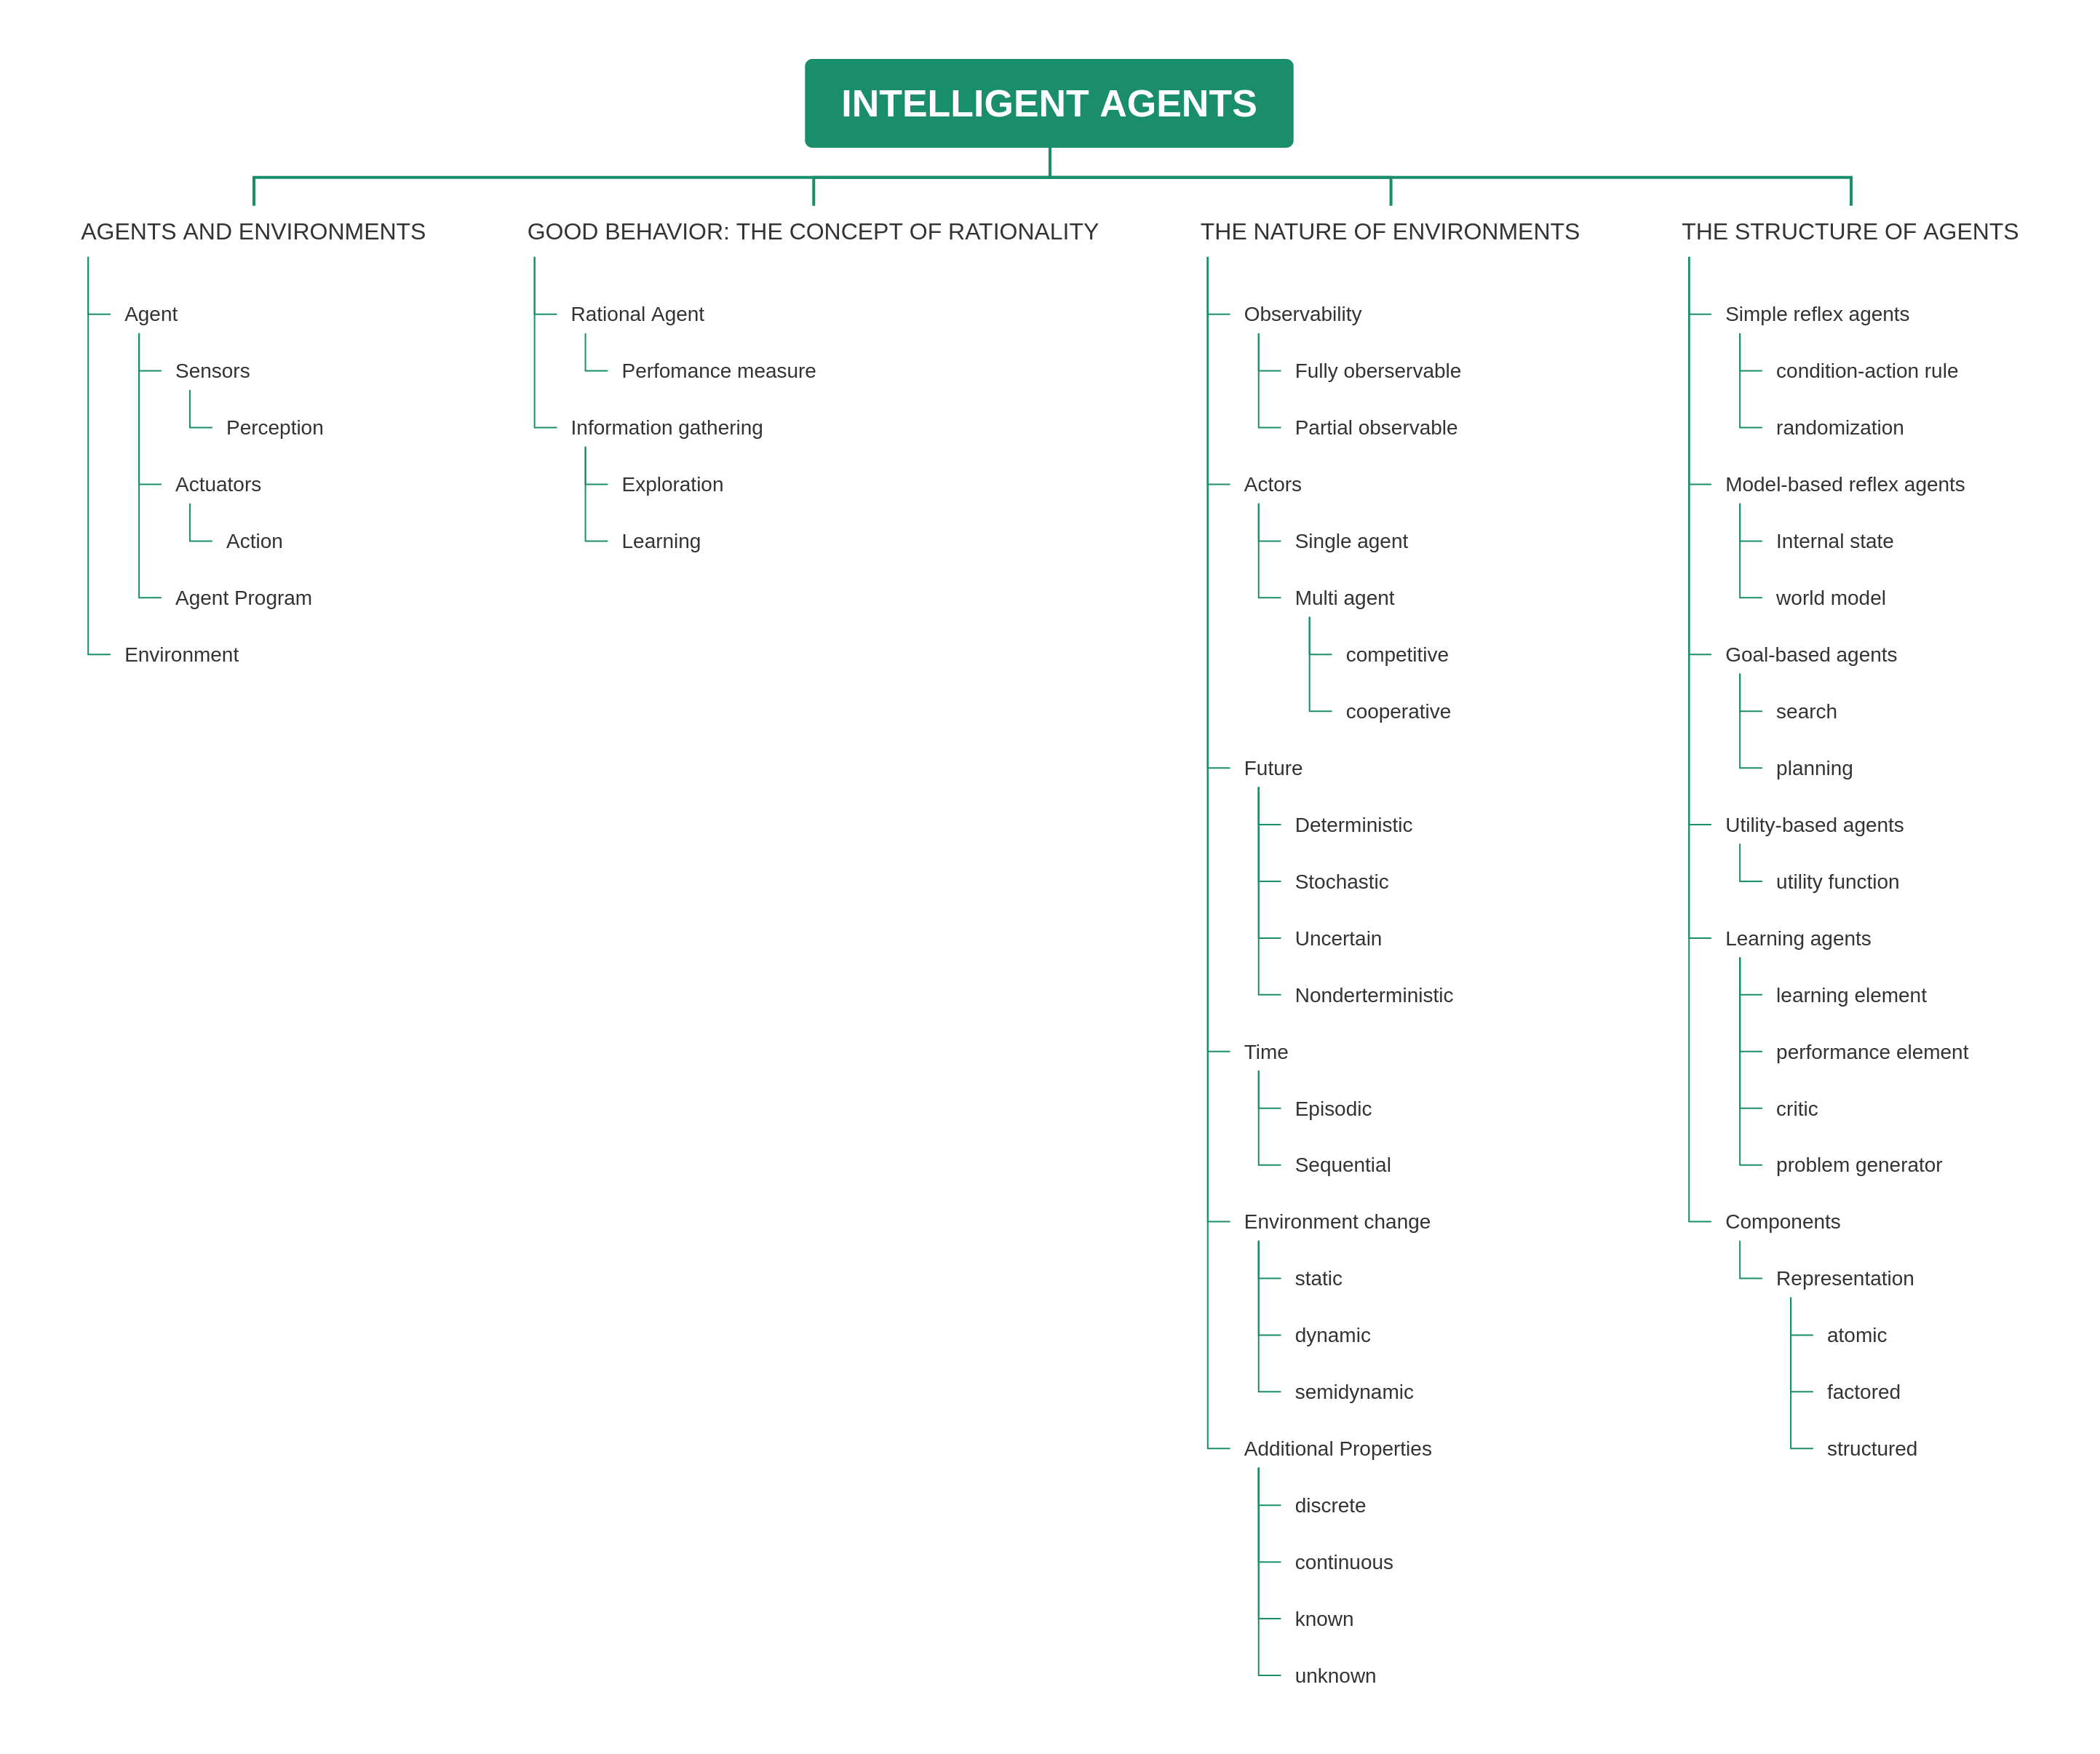
\includegraphics[width=\linewidth]{summary.png}
    \caption{Chapter 2 from \cite{russell_norvig_2014}}
    \label{fig:summary}
  \end{figure}
  


\section*{Task 2}
What are  \emph{reflex-, model-, goal-} and \emph{utility-based} agents? Answers based on \emph{Artificial intelligence: a modern approach} \cite{russell_norvig_2014} 

\begin{description}
    \item[reflex-based agent] 
    The simplest kind of agent. \
    A reflex-based agents looks up a action based only on current percepted input. 
    The behavior of this agent can be written as \textbf{condition-action} rules.
    
    \item[model-based agent] 
    This agent has the ability to create a \textbf{world model} for keeping track of external state.
    The agents perception is used to update the world model. Besides the state of the world, 
    the agent also model what each action can do. Based on this world state and the current 
    state it chooses the next action in the same way as the reflex-based agent.

    \item[goal-based agent] This agent models the external state the same way as the model-based \
    agent but the big difference is the introduction of goals. Those goals are used to
    choose the next action instead of the condition-action rules. For archiving its goals,
    this agent needs to \textbf{plan} ahead and \textbf{search} for the best action sequence.
 
    \item[utility-based agent]
     A goal based agents can only decide in a binary way if the goal is fulfilled. 
     This utility-based agent has an inbuilt \textbf{performance measurement} estimating how good the next 
     actions in the context of fulfilling its goal are.
  \end{description}


\section*{Task 3}
\emph{"Braitenberg vehicles are simple autonomous agents that move around based on sensor input."}\cite{harmendeweerd:1} With clever combinations
 Braitenberg was able to create simple behaviour patterns like light seeking or circling around objects. 
 By just attaching a sensor to an actuator. Check this website for a cool simulation\cite{harmendeweerd:1}. 
 Because no computation happens and each action is directly correlated to a specific sensorial input, 
 I would classify those agents as \textbf{reflex-based}.

\section*{Task 4}
Bring 3 nuns and 3 cannibals to the other side of a river without the nuns snacking on the cannibals. 
\subsection*{Task 4.a}
To describe the state of one iteration we have to know the count of nuns and cannibals on each side, 
as well as on which side the boat is.
\begin{verbatim}
  [|nuns|] [|cannibals|] [boat position] [|nuns|] [|cannibals|]
  for example: 3 3 R 0 0 
The boat is on the right side with 3 Nuns and 3 cannibals.
\end{verbatim}

\subsection*{Task 4.b}
\begin{enumerate}    
    \item 3 3 L 0 0
    \item 2 2 R 1 1
    \item 3 2 L 0 1
    \item 3 0 R 0 3
    \item 3 1 L 0 2
    \item 1 1 R 2 2
    \item 2 2 L 1 1
    \item 0 2 R 3 1
    \item 0 3 L 3 0
    \item 0 1 R 3 2
    \item 0 2 L 3 1
    \item 0 0 R 3 3
  \end{enumerate}

\subsection*{Task 4.c}
See the solution at Figure \ref{fig:nuns}. A \emph{red border} around a node means a forbidden state, 
a \emph{blue arrow} indicates an already found state. I could not explore to complete problem space because of some time constraints. 


Yes, it is important to check for repeated states because it saves steps - as soon as we find a repeated state we can just continue on 
the first occurrence.



\begin{figure}[h!]
  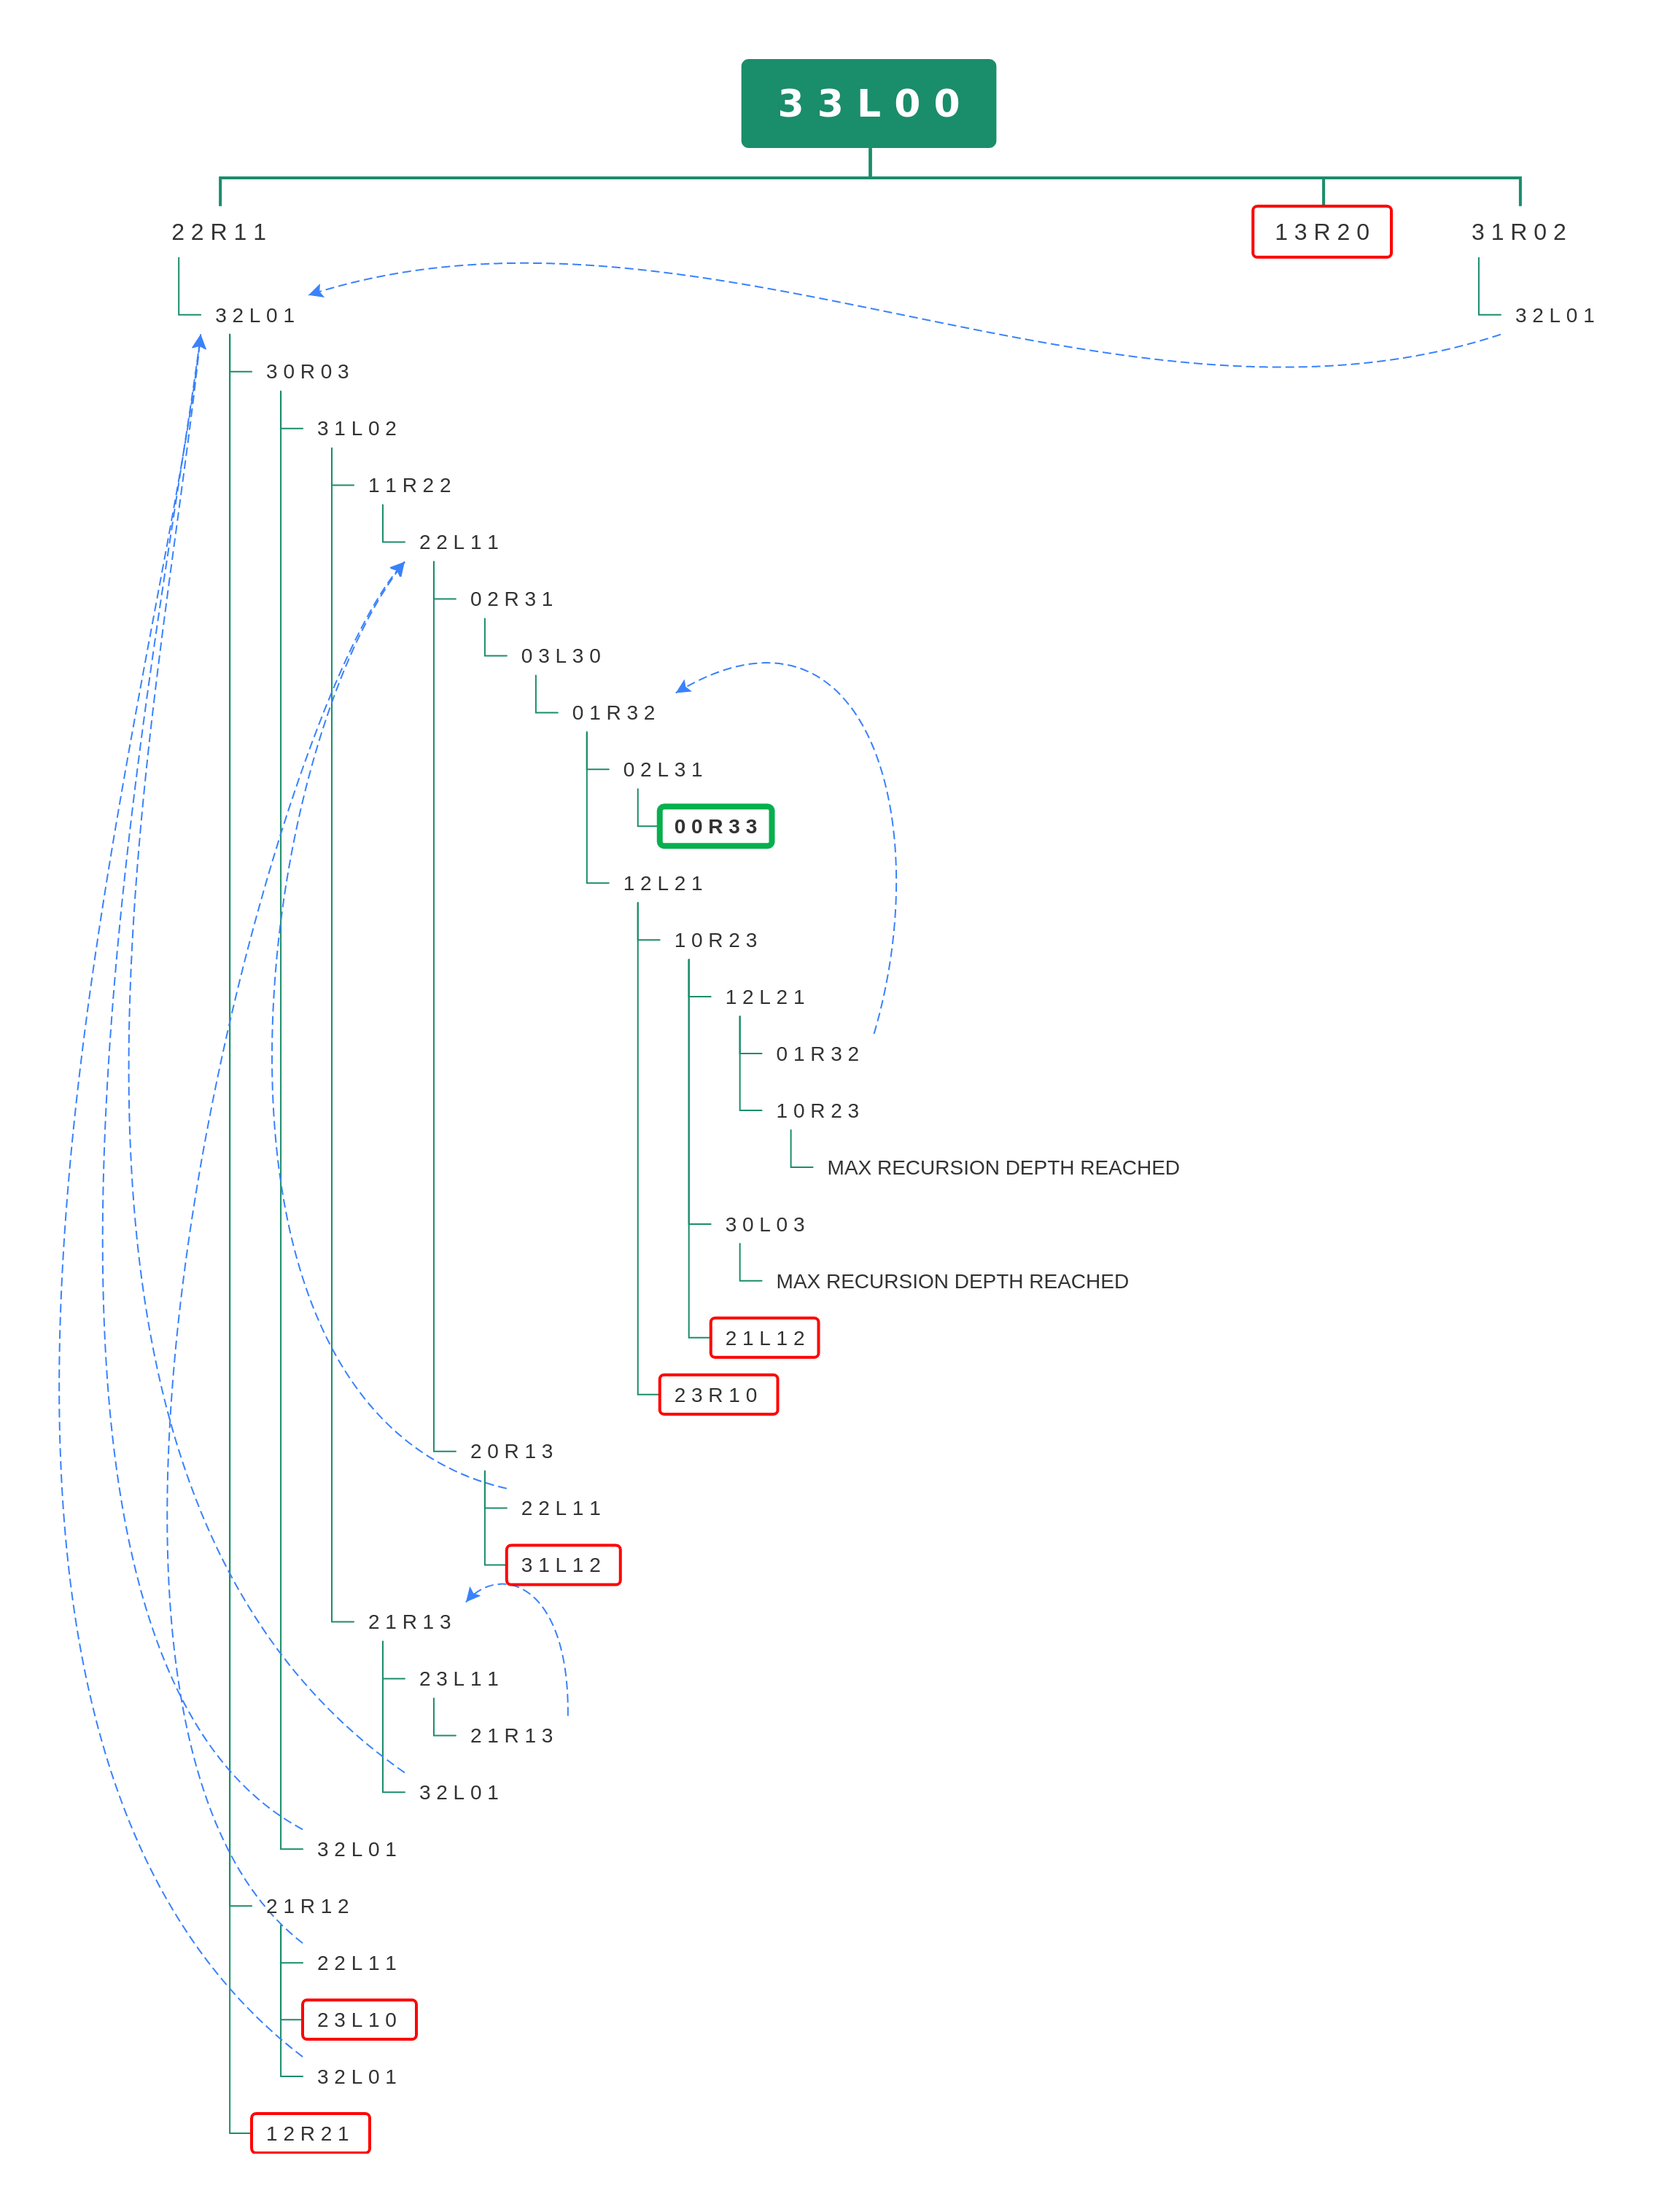
\includegraphics[width=\linewidth]{nuns.png}
  \caption{A subsection of the problem space. Terminates at node with green border.}
  \label{fig:nuns}
\end{figure}


\bibliography{stuff} 
\bibliographystyle{ieeetr}

\end{document}